%%%%%%%%%%%%%%%%%%%%%%%%%%%%%%%%%%%%%%%%%%%%%%%
\chapter{Generalized combination Network $(\epsilon,l)-\mathcal{N}_{h,r,s}$} \label{chap:general_network}
%%%%%%%%%%%%%%%%%%%%%%%%%%%%%%%%%%%%%%%%%%%%%%%

\section{Description \label{sec:Description_GCN}}

A generalized combination network $(\epsilon,l)-\mathcal{N}_{h,r,s}$
consists of 3 components from top to bottom: ``Source'' in the first
layer, ``Node'' in the middle layer, and ``Receiver'' in the third
layer. The network has a source with $h$ messages, $r$ nodes, and
$\left(\begin{array}{c}
r\\
\alpha
\end{array}\right)$ receivers, which form a single source multicast network modeled as
a finite directed acyclic multigraph. The source connects to each
node by $l$ parallel links and each node also connects to a receiver
by $l$ parallel links, which are respectively called a node's incoming
and outgoing edges. Each receiver is connected by $s$ links in total,
specifically $\alpha l$ links from $\alpha$ nodes and $\epsilon$
direct links from the source, i.e. $s=\alpha l+\epsilon$. The combination
network in \cite{Riis:2006} is the $(0,1)-\mathcal{N}_{h,r,s}$ network
and the $(1,1)-\mathcal{N}_{h,r,s}$ network is called One-Direct
Link Combination Network. Theorem 1 shows our interest of relations
between the parameters $h,\alpha,\epsilon$ and $l$.
\begin{thm}
\label{nw_parameters}The $(\epsilon,l)-\mathcal{N}_{h,r,s}$ network
has a trivial solution if $l+\epsilon\geq h$, and it has no solution
if $\alpha l+\epsilon<h$. 

Proof: Following to the network coding max-flow min-cut theorem for
multicast networks, the maximum number of messages from the source
to each receiver is equal to the smallest min-cut between the source
and any receiver. For our considered network, $s$ links have to be
deleted to disconnect the source from the receiver, which implies
that the min-cut between the source and each receiver is at least
$s$. Hence, $h\leq s\Leftrightarrow h\leq\alpha l+\epsilon$ $\Square$

There exist at least $l+\epsilon$ disjoint links connected to each
receiver. If $l+\epsilon\geq h$, each receiver can always reconstruct
its requested messages on its links. Then we only need to do routing
to select paths for the network. $\Square$
\end{thm}
\begin{rem}
Following to Theorem \ref{nw_parameters}, we are interested in networks
parameters satisfying this condition: $l+\epsilon+1\leq h\leq\alpha l+\epsilon$.
\end{rem}
\begin{figure}[H]
\caption{The generalized network $(\epsilon,l)-\mathcal{N}_{h,r,s}$\label{fig:The-generalized-network}}

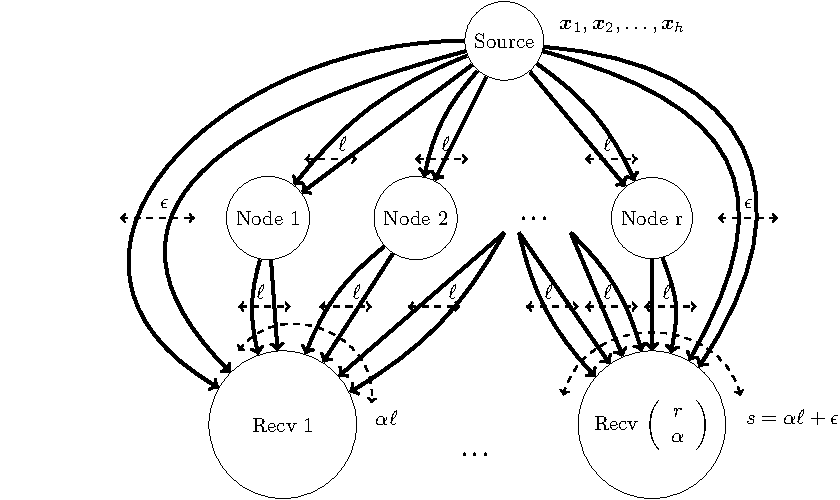
\includegraphics[width=0.5\paperwidth]{E:/Documents/TUM/THESIS/thesisCOD_Ha/figures/generalized_combination_nw}
\end{figure}

\begin{table}[H]
\caption{Parameters of network coding \label{tab:Parameters-of-network}}

\begin{tabular}{c|>{\centering}p{0.48\paperwidth}}
$h$ & The number of source messages\tabularnewline
\hline 
$r$ & The number of nodes in the middle layer\tabularnewline
\hline 
$\left(\begin{array}{c}
r\\
\alpha
\end{array}\right)$ & The number of receivers\tabularnewline
\hline 
$\ell$ & The source connects to each node by $\ell$ parallel links, and each
node also connects to one receiver by $\ell$ parallel links\tabularnewline
\hline 
$\alpha$ & A receiver is connected by any $\alpha$ nodes in the middle layer\tabularnewline
\hline 
$\epsilon$ & The source additionally connects to each receiver by $\epsilon$ direct
parallel links\tabularnewline
\hline 
$s$ & Each receiver is connected by $s$ links in total, with $s=\alpha\ell+\epsilon$.\tabularnewline
\end{tabular}
\end{table}


\section{Network coding for networks from this network family}

\subsection{Scalar network coding}

A message is equivalent to a symbol over $\ensuremath{\mathbb{F}}_{q_{s}}$.
As a network of the multicast model, all receivers request the same
packet of $h$ symbols at the same time \cite{Trautmann:2013}. A
packet is a 1-dimentional subspace of $\ensuremath{\mathbb{F}}_{q_{s}}^{h}$;
hence, each receiver must obtain a subspace of $\ensuremath{\mathbb{F}}_{q_{s}}^{h}$,
whose dimension is at least $h$, to be able to reconstruct the packet.
Through $\epsilon$ direct links connected from the source to a receiver,
the source can provide any required $\epsilon$ 1-dimensional subspaces
of $\ensuremath{\mathbb{F}}_{q_{s}}^{h}$ for the corresponding receiver.
Each receiver can accordingly reconstruct the packet if and only if
the linear span of $\alpha$ $l$-dimensional subspaces of $\ensuremath{\mathbb{F}}_{q_{s}}^{h}$
from the nodes is at least of dimension $h-\epsilon$. When this necessary
condition is satisfied, the network is said to have a \textit{solution}.
\begin{thm}
The $(0,1)-\mathcal{N}_{h,r,s}$ network has a solution if and only
if there exists an $\left(r,\left|\ensuremath{\mathbb{F}}_{q_{s}}\right|h,r-\alpha+1\right)$
$\left|\ensuremath{\mathbb{F}}_{q_{s}}\right|$-ary error correcting
code. \cite{Riis:2006}
\end{thm}

\subsection{Vector network coding}

The messages are vectors of length $t$ over $\ensuremath{\mathbb{F}}_{q}$.
Hence, a vector solution is over field size $q$ and dimension $t$.
Such a vector solution has the same alphabet size as a scalar solution
of field size $q^{t}$, and we denote $q_{v}=q^{t}$. A mapping from
the scalar solution of field size $q^{t}$ to a equivalent vector
solution is represented in Example \ref{ex:scalar_vector_mapping}.
Similarly with the scalar \textit{linear} coding solution, each receiver
can reconstruct its requested packet if and only if any $\alpha$
$\left(lt\right)$-dimensional subspaces span a subspace of dimension
at least $\left(h-\epsilon\right)t$.
\begin{thm}
A vector solution for the $(\epsilon,l)-\mathcal{N}_{h,r,s}$ network
exists if and only if there exists $\mathcal{G}_{q}\left(ht,lt\right)$
such that any $\alpha$ subspaces of the set span a subspace of dimension
at least $\left(h-\epsilon\right)t$. \cite{Zhang:2019}
\end{thm}

\subsection{Network as a matrix channel}

To formulate this description, the source has a set of disjoint messages
referred to packets which are either symbols from $\ensuremath{\mathbb{F}}_{q_{s}}$
(scalar coding) or vectors of length $t$ over $\ensuremath{\mathbb{F}}_{q}$
(vector coding). Each link in the network carries functions of the
packets, and a \textit{network code} is a set of these functions.
The network code is called \textit{linear} if all the functions are
linear and nonlinear otherwise. Each receiver $R_{j},j\in\left\{ 1,\ldots,N\right\} $
requests a subset of the source's length-$h$ messages, and this subset
is called a \textit{packet}. Through all the functions on the links
from the source to each receiver, the receiver obtains several linear
combinations of the $h$ messages to form a linear system of equations
for its requested packets. The coefficients of a linear combination
are called \textit{global coding vectors}. The linear equation system
that any receiver $R_{j}$ has to solve is as following:

\begin{equation}
\begin{array}{c|c}
Scalar & Vector\\
\underset{\ensuremath{\mathbb{F}}_{q_{s}}^{s}}{\underbrace{\left[\begin{array}{c}
y_{j_{1}}\\
\vdots\\
y_{j_{s}}
\end{array}\right]}}=\underset{\ensuremath{\mathbb{F}}_{q_{s}}^{s\times h}}{\underbrace{\boldsymbol{A}_{j}}}\cdot\underset{\ensuremath{\mathbb{F}}_{q_{s}}^{h}}{\underbrace{\left[\begin{array}{c}
x_{1}\\
\vdots\\
x_{h}
\end{array}\right]}} & \underset{\ensuremath{\mathbb{F}}_{q}^{st}}{\underbrace{\left[\begin{array}{c}
\underline{y}_{j_{1}}\\
\vdots\\
\underline{y}_{j_{s}}
\end{array}\right]}}=\underset{\ensuremath{\mathbb{F}}_{q}^{st\times th}}{\underbrace{\boldsymbol{A}_{j}}}\cdot\underset{\ensuremath{\mathbb{F}}_{q}^{th}}{\underbrace{\left[\begin{array}{c}
\underline{x}_{1}\\
\vdots\\
\underline{x}_{h}
\end{array}\right]}}
\end{array}\label{eq:linear_system}
\end{equation}

The transfer matrix $\boldsymbol{A}_{j}$ contains the links' \textit{global
coding vectors}, which are combined by the coefficients of linear
combinations on $\alpha l$ links from $\alpha$ nodes and $\epsilon$
direct-links to the corresponding receiver $R_{j}$:

\[
\begin{array}{c|c}
Scalar & Vector\\
\boldsymbol{A}_{j}=\left[\begin{array}{c}
\underline{a}_{j_{1}}\\
\vdots\\
\underline{a}_{j_{\alpha l}}\\
\vdots\\
\underline{a}_{j_{\alpha l+\epsilon}}
\end{array}\right] & \boldsymbol{A}_{j}=\left[\begin{array}{c}
\boldsymbol{A}_{j_{1}}\\
\vdots\\
\boldsymbol{A}_{j_{\alpha l}}\\
\vdots\\
\boldsymbol{B}_{j_{\alpha l+\epsilon}}
\end{array}\right]
\end{array}
\]

In general, the network is represented as a matrix channel for both
scalar and vector coding:
\begin{defn}
Network As Matrix Channel

The channel output can be written as: $\boldsymbol{Y}_{j}=\boldsymbol{A}_{j}\cdot\boldsymbol{X}$
\end{defn}
Because we reconstruct $\boldsymbol{X}$ with knowing $\boldsymbol{A}_{j}$,
i.e. the network structure is known, our network is coherent. A network
is \textit{sovable} or a network code is a \textit{solution}, if each
receiver can reconstruct its requested messages or solve the system
with a unique solution for scalars $x_{1},\ldots,x_{h}$, or vectors
$\underline{x}_{1},\ldots,\underline{x}_{h}$. Therefore, we want
to find global coding vectors such that the matrix $\boldsymbol{A}_{j}$
has full-rank for every $j=1,\ldots,N$, and such that $q_{s}$ or
$q^{t}$ is minimized. In Example \ref{ex:scalar_vector_mapping},
we provide a vector solution of field size $q$ and dimension $t$,
which has the same alphabet size as a scalar solution of field size
$q^{t}$
\begin{example}
\label{ex:scalar_vector_mapping} 

Given $h=3,q=2,t=2$, we consider the extension field $\ensuremath{\mathbb{F}}_{q^{t}=2^{2}}$.
The example shows how mapping messages from scalar coding to vector
coding.
\end{example}
\begin{figure}[H]
\caption{The mapping of scalar solution over $\ensuremath{\mathbb{F}}_{q_{s}=q^{t}}$
to the equivalen vector solution\label{fig:x_mapping}}

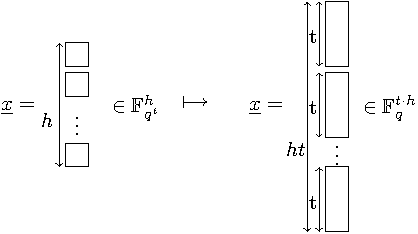
\includegraphics[width=0.3\paperwidth]{E:/Documents/TUM/THESIS/thesisCOD_Ha/figures/x_mapping}
\end{figure}

\begin{example}
We use the table of the extension field $\ensuremath{\mathbb{F}}_{2^{2}}$
with the primitive polynomial $f(x)=x^{2}+x+1$:
\end{example}
\begin{tabular}{|c|c|c|}
\hline 
power of $\alpha$ & polynomial & binary vector\tabularnewline
\hline 
- & 0 & 00\tabularnewline
\hline 
$\alpha^{0}$ & 1 & 01\tabularnewline
\hline 
$\alpha^{1}$ & $\alpha$ & 10\tabularnewline
\hline 
$\alpha^{2}$ & $\alpha+1$ & 11\tabularnewline
\hline 
\end{tabular}

For scalar coding, the messages are $x_{1},\ldots,x_{h=3}\in\ensuremath{\mathbb{F}}_{2^{2}}$
, and for vector coding the messages are $\underline{x}_{1},\ldots,\underline{x}_{h=3}\in\ensuremath{\mathbb{F}}_{2}^{2}$.
From the polynomial column, let's choose arbitrarily a scalar vector
$\underline{x}_{scalar}=(x_{1},x_{2},x_{3})=(1,\alpha,\alpha+1)$.
Then, we map it to $\underline{x}_{vector}=(\underline{x}_{1},\underline{x}_{2},\underline{x}_{3})$
by using the binary vector column as following:

\[
\left[\begin{array}{c}
x_{1}=1\\
x_{2}=\alpha\\
x_{3}=\alpha+1
\end{array}\right]\mapsto\left[\begin{array}{c}
\left(\begin{array}{c}
1\\
0
\end{array}\right)\\
\left(\begin{array}{c}
0\\
1
\end{array}\right)\\
\left(\begin{array}{c}
1\\
1
\end{array}\right)
\end{array}\right],
\]

where we use the following rule for mapping $x_{i}$ individually:
$a_{0}\cdot\alpha^{0}+a_{1}\cdot\alpha^{1}+\ldots+a_{t-1}\cdot\alpha^{t-1}\mapsto\left(\begin{array}{c}
a_{0}\\
a_{1}\\
\vdots\\
a_{t-1}
\end{array}\right)$.

To summarize the notations of both scalar and vector coding, we represent
them in the Table~\ref{tab:notations}:

\begin{table}[H]
\caption{Notations of network coding}

\label{tab:notations} 

\begin{tabular}{|>{\centering}p{0.2\paperwidth}|c|c|}
\hline 
 & Scalar Coding & Vector coding\tabularnewline
\hline 
\hline 
Source Messages/Packets & $\begin{array}{c}
x_{1},\ldots,x_{h}\in\ensuremath{\mathbb{F}}_{q_{s}}\\
\underline{x}\in\ensuremath{\mathbb{F}}_{q_{s}}^{h}
\end{array}$ & $\begin{array}{c}
\underline{x}_{1},\ldots,\underline{x}_{h}\in\ensuremath{\mathbb{F}}_{q}^{t}\\
\underline{x}\in\ensuremath{\mathbb{F}}_{q}^{th}
\end{array}$\tabularnewline
\hline 
Global Coding Vectors Of Receiver $R_{j}$ & $\underline{a}_{j_{1}},\ldots,\underline{a}_{j_{s}}\in\ensuremath{\mathbb{F}}_{q_{s}}^{h}$ & $\boldsymbol{A}_{j_{1}},\ldots,\boldsymbol{A}_{j_{s}}\in\ensuremath{\mathbb{F}}_{q}^{t\times th}$\tabularnewline
\hline 
Transfer Matrix Of Receiver $R_{j}$ & $\boldsymbol{A}_{j}\in\ensuremath{\mathbb{F}}_{q^{t}}^{s\times h}$ & $\boldsymbol{A}_{j}\in\ensuremath{\mathbb{F}}_{q}^{st\times th}$\tabularnewline
\hline 
Packets On Receiver $R_{j}$ & $\begin{array}{c}
y_{j_{1}},\ldots,y_{j_{s}}\in\ensuremath{\mathbb{F}}_{q_{s}}\\
\underline{y}\in\ensuremath{\mathbb{F}}_{q_{s}}^{s}
\end{array}$ & $\begin{array}{c}
\underline{y}_{j_{1}},\ldots,\underline{y}_{j_{s}}\in\ensuremath{\mathbb{F}}_{q}^{t}\\
\boldsymbol{Y}_{j}\in\ensuremath{\mathbb{F}}_{q}^{st}
\end{array}$\tabularnewline
\hline 
Number of nodes & $r_{scalar}$ & $r_{vector}$\tabularnewline
\hline 
\end{tabular}
\end{table}

\begin{rem}
By using the vector coding, the upper bound number of solutions increases
from $q^{tkh}$ to $q^{t^{2}kh}$. Therefore, vector network coding
offers more freedom in choosing the coding coefficients than does
scalar linear coding for equivalent alphabet sizes, and a smaller
alphabet size might be achievable \cite{Ebrahimi2011}. By this advantage,
we can have higher amount of receivers, i.e. higher amount of nodes,
in vector network coding.
\end{rem}

\subsection{Comparison between scalar and vector solutions by the gap size}

The \textit{gap} represents the difference between the smallest field
(alphabet) size for which a scalar linear solution exists and the
smallest alphatbet size for which we can construct a vector solution.
In this study, we define a solvable vector network coding over the
field size $\ensuremath{\mathbb{F}}_{q}^{t}$, and we conjecture the
minimum amount of nodes such vector solution can achieve, i.e. $r_{vector}\geq f_{1}(q)$,
with $f_{1}:\mathbb{Z}\mapsto\mathbb{Z}$. Meanwhile, we has a scalar
solution for the same network existing if and only if: $r_{scalar}\leq f_{2}\left(q_{s}\right)$,
with $f_{2}:\mathbb{Z}\mapsto\mathbb{Z}$. To find the field size
$q_{s}$ required for a scalar solution to reach the minimum achievable
vector solution's nodes in this setting, we consider $r_{max,scalar}=f_{2}\left(q_{s}\right)=f_{1}(q)=r_{min,vector}$.
Finally, we calculate the gap by $g=q_{s}-q_{v}=q_{s}-q^{t}.$ Throughout
this study, we show that vectors solutions significantly reduce the
required alphabet size by this gap. 

\section{Special cases of generalized combination network}

\subsection{The $(l-1)$-Direct Links and $l$-Parrallel Links $\mathcal{N}_{h=2l,r,s=3l-1}$}

This subfamily contains the largest number of direct links from the
source to the receivers. For $l\geq2$, this network $\left(\epsilon=l-1,l\right)-\mathcal{N}_{h=2l,r,s=3l-1}$
yields the gap $q^{(l-1)t^{2}/l+\mathcal{O}(t)}$ between vector solutions
and optimal scalar solutions. The vector solution is based on an $\mathcal{MRD}\left[lt\times lt,t\right]_{q}$
code. Further, the gap tends to $q^{t^{2}/2+\mathcal{O}(t)}$ for
large $l$.
\begin{lem}
There is a scalar linear solution of field size $q_{s}$ for the $\left(\epsilon=l-1,l\right)-\mathcal{N}_{h=2l,r,s=3l-1}$
network, where $l\geq2$, if and only if $r\leq\left[\begin{array}{c}
2l\\
l
\end{array}\right]_{q_{s}}$.
\end{lem}

\subsection{The 1-Direct Link and $l$-Parrallel Links $\mathcal{N}_{h=2l,r,s=2l+1}$}

This is the smallest direct-link subfamily has an vector solution
outperforming the optimal scalar solution, i.e. an vector solution
outperforming the optimal scalar has not yet been found for the network
$(0,l>1)-\mathcal{N}_{h,r,s}$. Similar to the previous subfamily
$\left(\epsilon=l-1,l\right)-\mathcal{N}_{h=2l,r,s=3l-1}$, when $l\geq2$
or $h\geq4$, this network yields the largest gap $q^{t^{2}/2+\mathcal{O}(t)}$
in the alphabet size by using the same approach with an $\mathcal{MRD}\left[lt\times lt,(l-1)t\right]_{q}$
code. 

\subsection{The $\epsilon$-Direct Links $\mathcal{N}_{h,r,s}$}

This subfamily is denoted as $\left(\epsilon\geq1,l=1\right)-\mathcal{N}_{h,r,s}$
and is the most focus topic on this thesis, because it motivates some
interesting questions on a classic coding problem and on a new type
of subspace code problem. In the chapter 3, we show our largest code
set with low number of subspace codes for the network $\left(\epsilon=1,l=1\right)-\mathcal{N}_{h=3,r,s=4}$.

\subsection{The $\left(\epsilon=0,l=1\right)-\mathcal{N}_{h,r,s}$ Combination
Network}

Since the scalar solution for the combination network uses an $MDS$
code, a vector solution based on subspace codes must go beyond the
$MDS$ bound, i.e. Singleton bound $d\leq n-k+1$, to outperform the
scalar one. In paper \cite{Wachter-Zeh:2018}, it is proved that vector
solutions based on subspace codes cannot outperform optimal scalar
linear solutions for $h=2$, and they conjecture it for all $h$.
Unfortunately, a vector solution based on an $\mathcal{MRD}\left[t\times t,t\right]_{q}$
code is also proved that it cannot outperform the optimal scalar linear
solution.

\subsection{The 2 networks yields gap $q^{(h-3)t^{2}/(h-1)+\mathcal{O}(t)}$}

For $h=2l-1$: $\left(\epsilon=l-2,l\right)-\mathcal{N}_{h=2l-1,r,s=3l-2}$

For $h=2l+1$: $\left(\epsilon=l-1,l\right)-\mathcal{N}_{h=2l+1,r,s=3l-1}$

\clearpage